\documentclass{beamer-control}
\usepackage{beamer-control-singlefile}
\INCLUDEONLY{Modelling Methodology}
\begin{document}
\CONCEPT{Modelling Methodology}

\begin{SUMMARY}
\begin{itemize}
\item Block diagrams
\item Modelling from experiments
\begin{itemize}
\item ITD, FOTD, SOTD models
\item Estimating models from data
\end{itemize}
\item Normalisation and scaling
\end{itemize}
\vfill References:
\begin{itemize}
\item \astrom{§3.3}
\end{itemize}
\end{SUMMARY}



\SUBCONCEPT{Block diagram}

\begin{frame}{The block diagram}
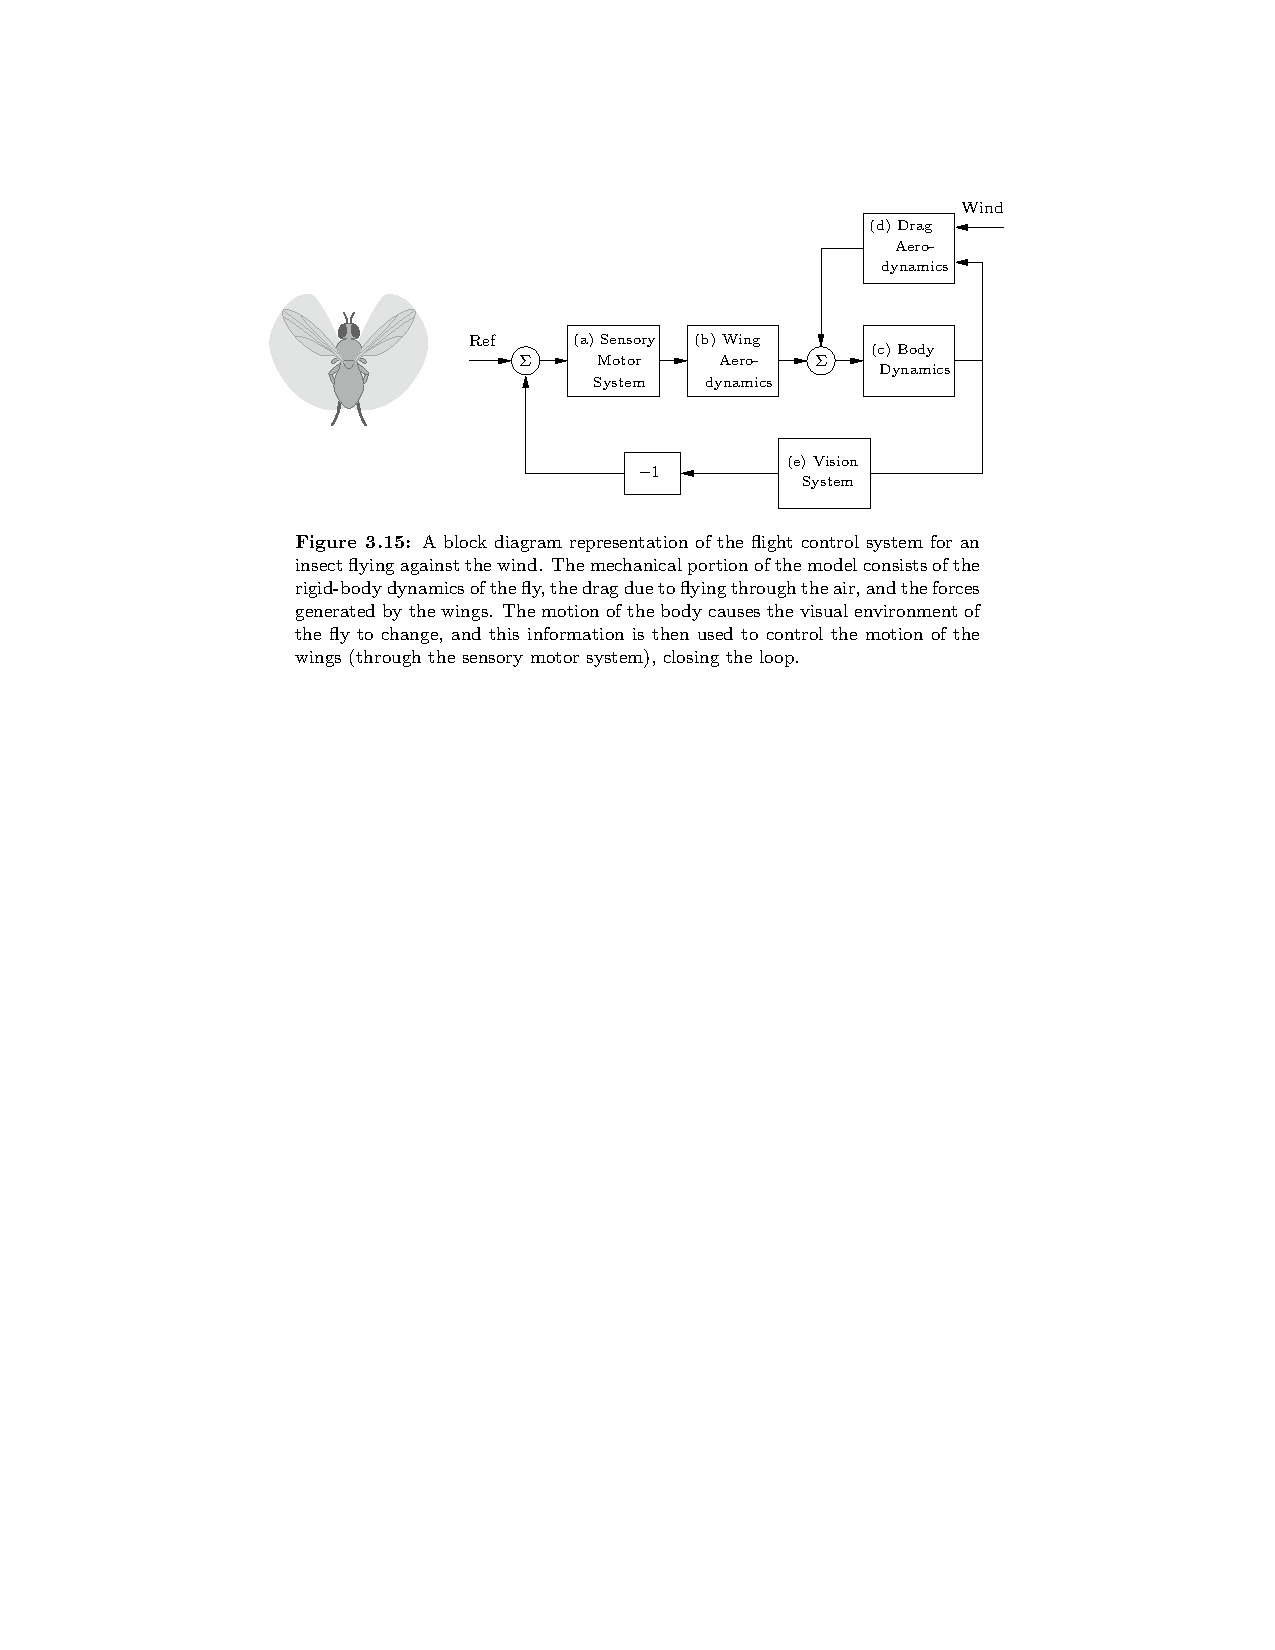
\includegraphics[width=\linewidth]{figure3.15}
\end{frame}

\begin{frame}
\frametitle{Block diagram elements}
\framesubtitle{Refer \AMref{Figure 3.14}}
\begin{itemize}
\item<alert@1> Sources/sinks
\item<alert@2> Summation
\item<alert@3> Gain
\item<alert@4> Function
\item<alert@5> Derivative
\item<alert@6> Integral
\item<alert@7> Saturation
\end{itemize}
\end{frame}

\begin{frame}
\frametitle{Block diagram of a controller}
\begin{align}
\Deriv{x}{t} &= f(x,u) & y &= h(x) & u &= -ky
\end{align}
\vspace*{0pt plus 1 filll}
\null
\end{frame}


\SUBCONCEPT{Modelling from experiments}

\begin{frame}
\frametitle{Integrator with Time Delay (ITD)}
\begin{columns}
\column{0.4\textwidth}
\only<1>{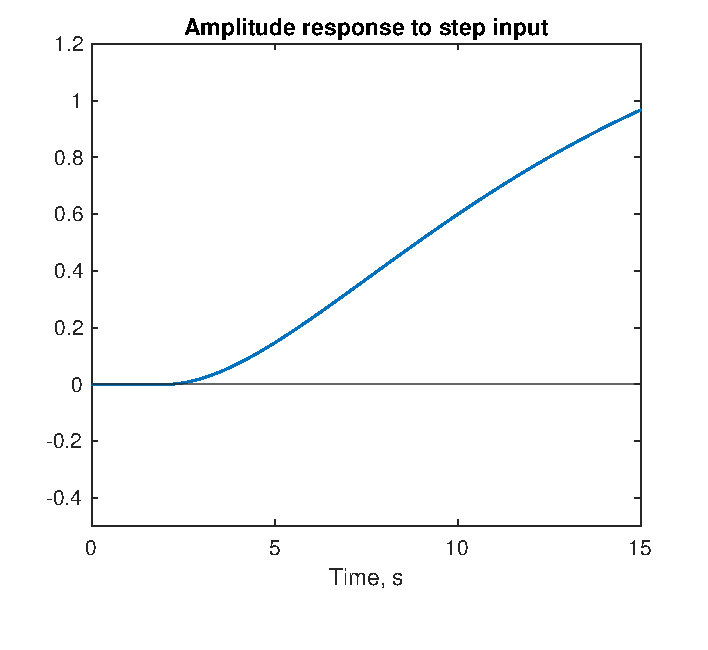
\includegraphics[width=1.3\linewidth]{itd}}%
\only<2>{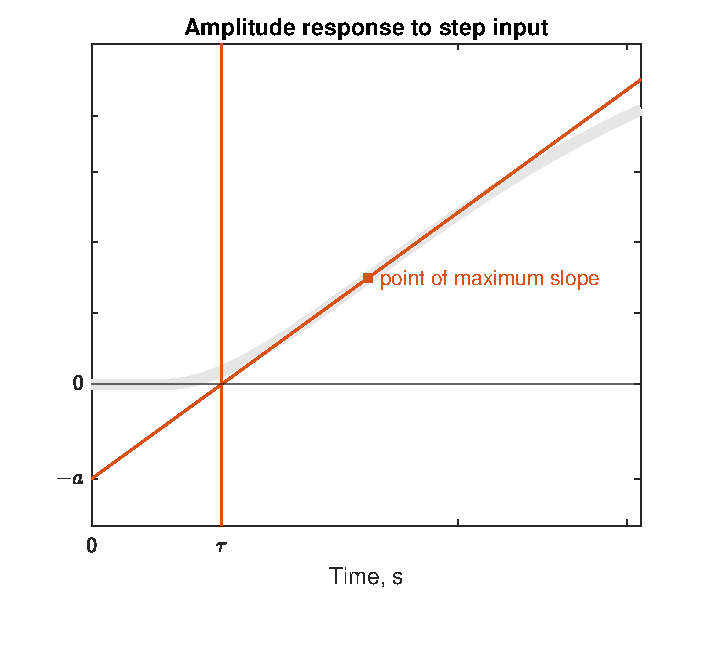
\includegraphics[width=1.3\linewidth]{itd-at}}%

\column{0.55\textwidth}
\scriptsize
\begin{uncoverenv}<2>
\begin{itemize}
\item Time delay $\TimeDel$ and intercept $-a$: extrapolate from point of maximum slope
\end{itemize}
\end{uncoverenv}
\end{columns}
\end{frame}

\begin{frame}{First Order system with Time Delay (FOTD)}
\begin{columns}
\column{0.4\textwidth}
\only<1>{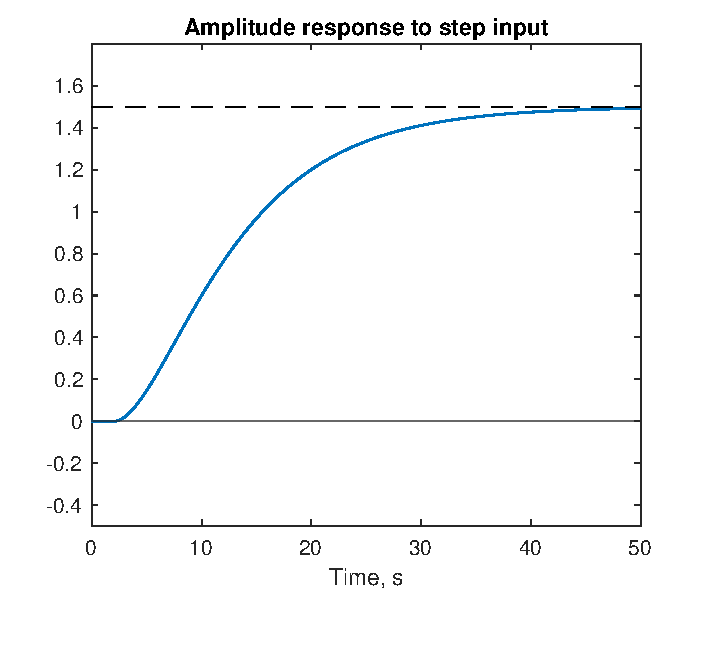
\includegraphics[width=1.3\linewidth]{fotd}}%
\only<2>{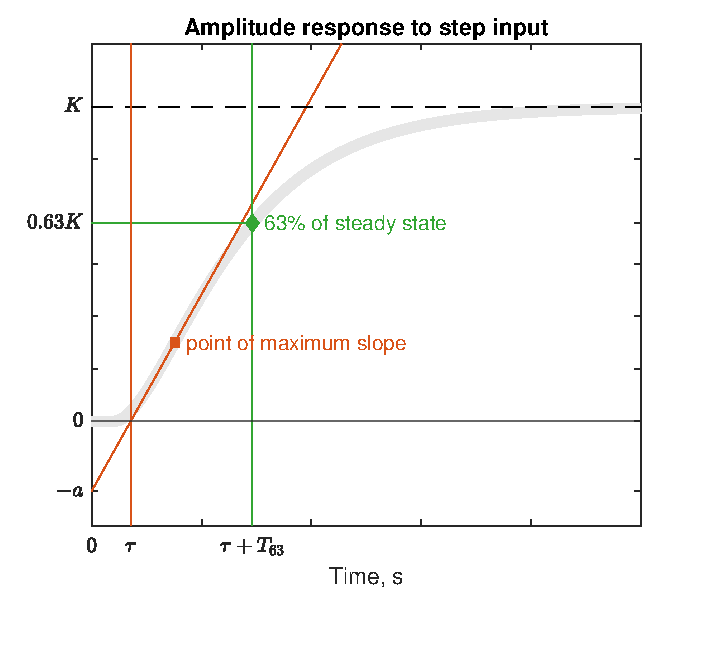
\includegraphics[width=1.3\linewidth]{fotd-LT}}%

\column{0.55\textwidth}
\scriptsize
\begin{uncoverenv}<2>
\begin{itemize}
\item Time delay $\TimeDel$ and intercept $-a$: extrapolate from point of maximum slope
\item Time constant $\TimeConst_{63}$: from 63\% of steady state value
\end{itemize}
\end{uncoverenv}
\end{columns}
\end{frame}


\begin{frame}{Second Order system with Time Delay (SOTD)}
\begin{columns}
\column{0.4\textwidth}
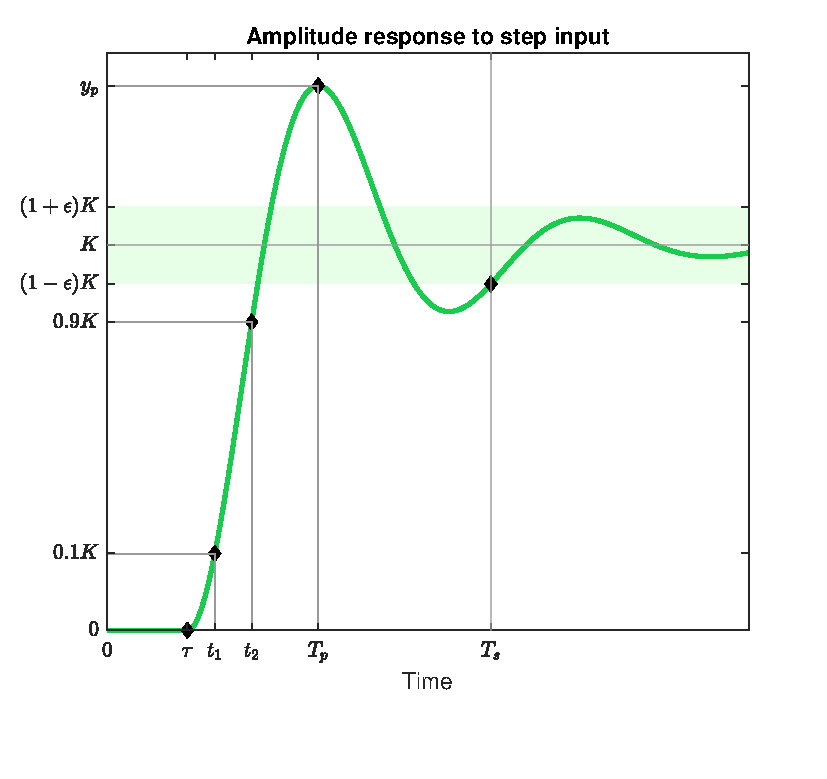
\includegraphics[width=1.3\linewidth]{sotd-annot}

\column{0.55\textwidth}
\scriptsize
\begin{itemize}
\item Steady state (equilibrium) response $\StaticGain$: $\StaticGain=1$ for zero steady state error
\item Peak response $y_p$ at peak time $T_p$
\item Overshoot $(y_p-\StaticGain)/\StaticGain$ [\%]: measure of dynamic error, increases with smaller damping ratio $\zz$
\item Rise time $t_2-t_1$: measure of the `speed'
\item Settling time $T_s$: another measure of the `speed'; $\epsilon$ usually 1\%, 2\%, or 5\%
\end{itemize}
\end{columns}
\end{frame}

\begin{frame}
\frametitle{Second order system relationships ($m\ddot q + c \dot q + kq = f$)}
Natural frequency $\wn$ and damping ratio $\zz$:
\begin{gather}
\wn = \sqrt{\frac{k}{m}} \qquad \zz = \frac{c}{2\sqrt{km}} 
\end{gather}
Resonance frequency:
\begin{align}
\wres = \wn\sqrt{1-2\zz^2}
\end{align}
Estimate resonance frequency $\wres$ with:
\begin{align}
\wres \approx \frac{2\pi}{T_2-T_1}
\end{align}
$T_{1,2}$ are times of successive local maxima in the step response.
\end{frame}

\begin{frame}
\frametitle{Estimating damping ratio}

The decay ratio $d$ often used to estimate the damping ratio
\begin{align}
d=\frac{y_2-\StaticGain}{y_1-\StaticGain}
\end{align}
where $y_{1,2}$ are the amplitudes of successive local maxima in the step response.
\bigskip

Estimate damping ratio $\zz$ with:
\begin{align}
  \zz \approx \frac{1}{\sqrt{1+\left(\frac{2\pi}{\ln d}\right)^2}}
\end{align}
\end{frame}

\begin{frame}
\frametitle{Estimating the remaining parameters (if needed)}
\begin{itemize}
\item
$\wn = \wres/\sqrt{1-2\zz^2} $
\item
$k = F_0/K$ --- Hooke's law
\item
$m$ follows from $\wn$
\item
$c$ follows from $\zz$
\end{itemize}
\end{frame}

\begin{frame}
\frametitle{Example}
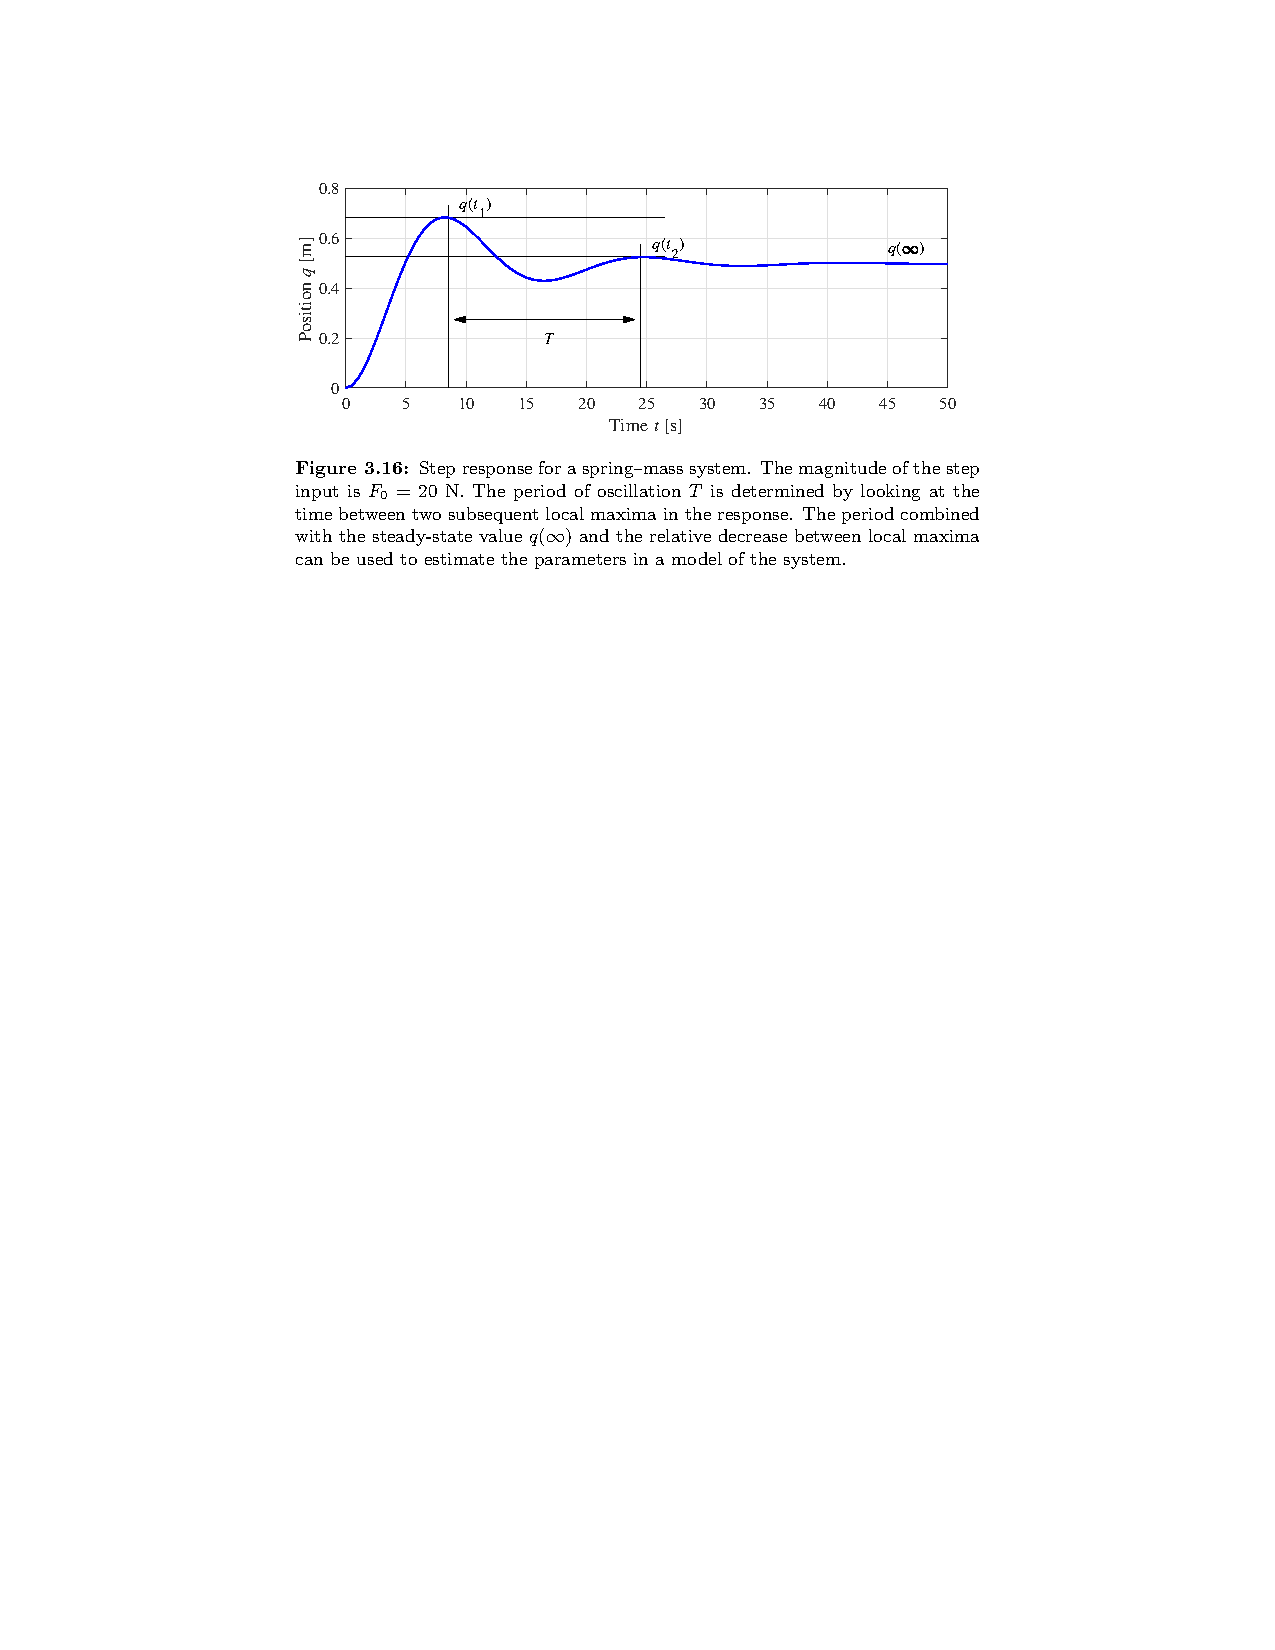
\includegraphics[width=\linewidth]{figure3.16}

\end{frame}

\begin{frame}
\frametitle{Example}
\begin{align}
t_2-t_1&\approx \SI{16}{s} & \therefore~ \wres &\approx \SI{0.4}{rad/s} \\
K &\approx \SI{0.5}{m},\quad F_0=\SI{20}{N} & \therefore~ k&\approx \SI{40}{N/m} \\
d&=\frac{y_2-\StaticGain}{y_1-\StaticGain}\approx\frac{\SI{0.16}{m}}{\SI{0.1}{m}}=16 & \therefore~ \zz&\approx0.40  \\
\wn &= \wres/\sqrt{1-2\zz^2} \approx \SI{0.33}{rad/s} & \therefore~ m &= k/\wn^2 = \SI{371}{kg} \\
&& \therefore~c &= 2\zz\sqrt{km} \approx \SI{98}{kg/s}
\end{align}
This is not the same as the textbook --- I expect my numbers were poorly estimated :)

\end{frame}


\SUBCONCEPT{Normalisation and Scaling}

\begin{frame}
\frametitle{Normalisation and Scaling}
\begin{itemize}
\item Where possible, normalise your systems
\item This will generalise the results and make it more likely that off-the-shelf control approaches will be valid
\item Some normalisations are rather mathematical\dots (see example in textbook)
\item Scaling of inputs and outputs is more straightforward:
\end{itemize}
\end{frame}

\begin{frame}
\frametitle{Normalisation}


\begin{figure}
  \centering
  \tikzset{%
    block/.style    = {
                        draw,
                        rectangle,
                        minimum height = 3em,
                        minimum width = 4em,
                        node distance=6em
                      },
    input/.style    = {coordinate},
    output/.style   = {coordinate}
  }

  \begin{tikzpicture}[auto, node distance=2cm, >=latex, thick]

    \draw
    node [input, name=R] {R}
    node [block, right of=R]     (G) {$G$}
    node [output,right of=G] (Y) {}
    ;

    \draw[->](R) -- node {$R$}(G);
    \draw[->](G) -- node {$Y$} (Y);

  \end{tikzpicture}
  \bigskip
  \caption{Plant $P = Y/R$.}
\end{figure}


\begin{figure}
  \centering
  \tikzset{%
    block/.style    = {
                        draw,
                        rectangle,
                        minimum height = 3em,
                        minimum width = 4em,
                        node distance=8em
                      },
    input/.style    = {coordinate},
    output/.style   = {coordinate}
  }

  \begin{tikzpicture}[auto, node distance=2cm, >=latex, thick]

    \draw
    node [input, name=R] {R}
    node [block, right of=R] (RR) {$r_{\mathrm{max}}$}
    node [block, right of=RR] (G) {$G$}
    node [block, right of=G] (YY) {$1/y_{\mathrm{max}}$}
    node [output,right of=YY] (Y) {}
    ;

    \draw[->](R) -- node {$\hat R$}(RR);
    \draw[->](RR) -- node {$R$}(G);
    \draw[->](G) -- node {$Y$} (YY);
    \draw[->](YY) -- node {$\hat Y$}(Y);

  \end{tikzpicture}
  \bigskip
  \caption{Plant $\hat P = \hat Y/\hat R$ with normalisation. (Often implicit, no `hats'.)}
\end{figure}

\end{frame}



\SUBCONCEPT{Examples}

\begin{frame}
\frametitle{Important!}
\begin{itemize}
\item Many of these concepts will be very abstract until you try some examples out
\item Please read through \AMref{§3.4 `Examples'} and try to replicate at least one of them in your own style (pen+paper, Matlab, etc.)
\end{itemize}
\end{frame}

\SUMMARYFRAME
\FINALE

\end{document}
